\chapter{Evaluation and Experimentation}

\section{Evaluation Metrics}

During the training and the final experiments, the agents are primarily evaluated based on the success rate, as well as the average completion time and the collision rate. Success rate is defined as the percentage of episodes in which the agent successfully completes the parcour. These metrics, which were previously used by \autocite{maximilian}, measure the agent behaviour's most important properties.

Additional metrics will be monitored during the training process to identify weak-points and erroneous behaviour of the agent. Monitoring the training process can provide insights into the agent's behaviour and aid in selecting appropriate hyperparameters. TensorBoard will be used to visualize the monitored metrics \ref{fig:tensorboard}.
These metrics may include be the average cumulative reward, the average number of passed goals, the average distance travelled, the average amount of collisions, the average game duration and the average speed of the agent.


\section{Experiments}

The proposed experiments build on the scenarios from \autocite{maximilian}. These experiments included three parcours with different difficulty levels \ref{fig:3tracks} and conducted 3 different experiments with each trained agent. The first experiment used the same settings as the simulation environment. The second experiment was conducted under different lighting settings. The third one changed the motor power of the agent's two front wheels. All experiments primarily used the success rate to evaluate the agent's performance, the success rate is the proportion of successfully completed parcours.

The first two experiments will be used in this thesis as well, using the same experiments allows for an easy comparison to the previous research. The experiment with varying motor power will be omitted, since it is not related to the research goals of this thesis.


\subsection{Research Question 1 - Is it possible to train an autonomous driving agent consisting of a convolutional neural network with end-to-end reinforcement learning to reliably solve the parcours of all difficulty levels?}

The experiments under minimal changes will be used to judge if the agent is able to reliably solve all parcours. \ref{fig:3tracks} shows three parcours of different difficulty levels, there are further variations of these parcours that change the positioning and colour of the obstacles. The parcours are evaluated using the success rate, if the agent is able to reliably solve all parcours the agent and training implementation can be considered successful.

\begin{figure}
    \centering
    \subfigure[Easy]{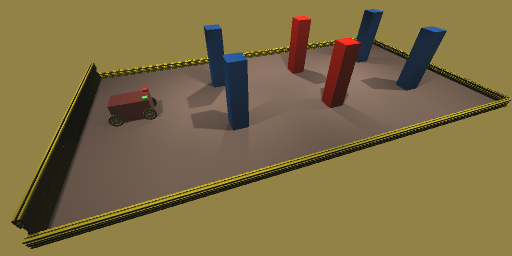
\includegraphics[width=0.3\textwidth]{Bilder/evaluation_easy.png}}\qquad
    \subfigure[Medium]{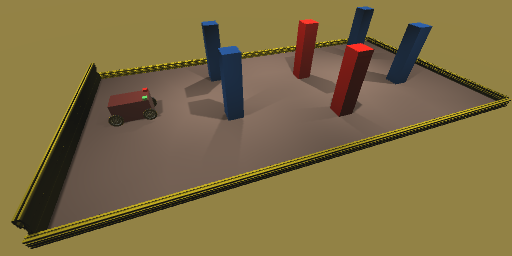
\includegraphics[width=0.3\textwidth]{Bilder/evaluation_medium.png}}\qquad
    \subfigure[Hard]{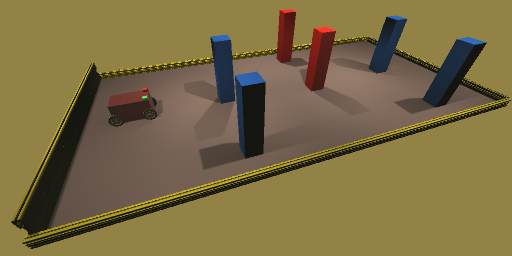
\includegraphics[width=0.3\textwidth]{Bilder/evaluation_hard.png}}\qquad
    \caption{Evaluation Tracks of different difficulties}
    \label{fig:3tracks}
\end{figure}

\subsection{Research Question 2 - Is it possible to use an end-to-end trained CNN to make the agent robust to changing light conditions?}

The evaluation parcours will be used with varying light settings to evaluate the agent's robustness towards changing light conditions. The agent's performance will be measured using the success rate, if the agent performs similarly across all light settings, the agent can be considered robust to changing light conditions.

\begin{figure}
    \centering
    \subfigure[Standard Lighting Agent POV]{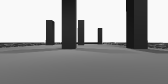
\includegraphics[width=0.3\textwidth]{Bilder/light_setting_pov_standard.png}}\qquad
    \subfigure[Standard Lighting Arena]{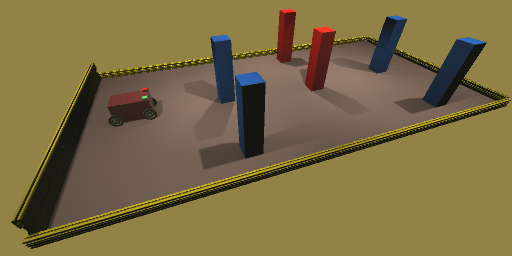
\includegraphics[width=0.4\textwidth]{Bilder/light_setting_arena_standard.png}}
    \subfigure[Reduced Lighting Agent POV]{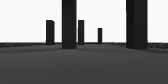
\includegraphics[width=0.3\textwidth]{Bilder/light_setting_pov_reduced_lighting.png}}\qquad
    \subfigure[Reduced Lighting Arena]{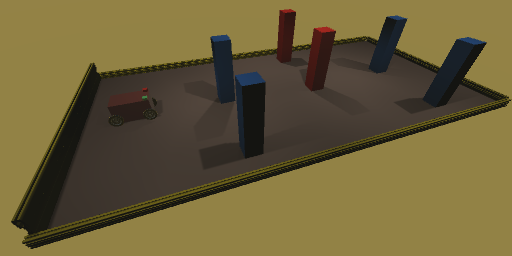
\includegraphics[width=0.4\textwidth]{Bilder/light_setting_arena_reduced_lighting.png}}
    \subfigure[Increased Lighting Agent POV]{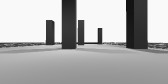
\includegraphics[width=0.3\textwidth]{Bilder/light_setting_pov_increased_lighting.png}}\qquad
    \subfigure[Increased Lighting Arena]{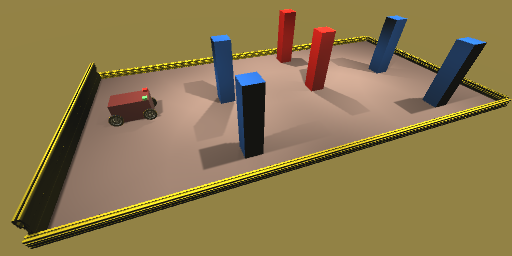
\includegraphics[width=0.4\textwidth]{Bilder/light_setting_arena_increased_lighting.png}}

    \caption{Agent Camera POV and Arena Screenshots of the different light settings} 
    \label{fig:light_settings}
\end{figure}

\subsection{Research Question 3 - Is it possible to use a neural network that can be transfered to a physical robot?}

To answer question 3, the developed agent will be evaluated on the JetBot's processing unit. There will be no physical experiments with the JetBot due to time constraints. Instead a replay of an evaluation parcour is generated in Python. The replay is then processed on the JetBot to measure its processing capabilities. The replay will consist of input-output pairs and metadata, such as processing times. If the JetBot is able to reproduce the behaviour from the replay at sufficient speed, the agent can be considered transferable to the JetBot.

% kann ich die Experimente mit varying motor power weglassen?
% die Experimente stehen nicht so stark im Zusammenhang mit den beiden Research goals
% ja